
\begin{figure}[t!]
\centering
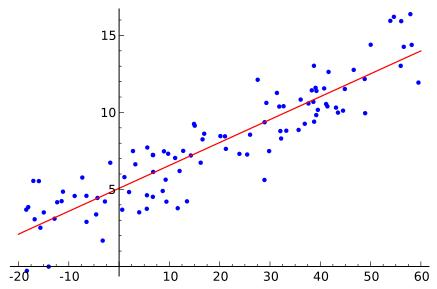
\includegraphics[width=10cm]{images/linear_regression.jpg}
\caption{Ejemplo de Regresión Lineal}
\end{figure}

\section{Análisis de regresión}

Llegado a este punto, dada una variable acústico-prosódica, nos interesó evaluar la relación entre el entrainment o mimetización sobre dicha variable y las distintas variables sociales. Con esto en mente, planteamos un modelo de regresión lineal tomando como nuestra variable \emph{explicativa} la mimetización, y la variable \emph{dependiente} será la variable social elegida. Este análisis de regresión nos permitió observar cuál es la variación conjunta de ellas.

Nuestra hipotesis consistió en que la mimetización (por ejemplo, en la intensidad o pitch) se relacionaría de manera directa con ciertas variables sociales de connotación positiva (por ejemplo, la compenetración en el juego) y que se relacionaría de manera inversa con aquellas de carácter negativo (el aburrimiento o el desagrado por su compañero), siguiendo la línea de trabajos previos \cite{gravano2015backward}. En la siguiente sección se describe el primer análisis, en el cual utilizamos el modelo ``pooled'' o agrupado, donde utilizamos todos los datos juntos indistintamente de la sesión y hablante del que provengan.
